%%%%%%%%%%%%%%%%%%%%%%%%%%%%%%%%
\section{Results} \label{S:results}
%%%%%%%%%%%%%%%%%%%%%%%%%%%%%%%%
%
%###############################
\subsection{About the variability of the data} \label{sS:results_variability}
%###############################
%
As expected, our data registered three levels of variability: between blocks and children variability, and finally, the entropy replicates variability.

Evidence from the posterior estimates reveal the block random effects explained a small amount of variability in the data ($\sigma_{b}=0.26$, top panel of figure \ref{fig:variability}), and its inclusion/exclusion in the model did not change the parameter estimates. The previous implied the experiment was correctly `set up', as the series in which the utterances were transcribed did not explain a significant amount of variation, nor its exclusion biased the parameter estimates.

On the contrary, we observe a significantly larger variability between children. More precisely, the \textit{speech intelligibility} variability between children was more than three times the block effects variability ($\sigma_{i}=0.74$, middle panel of figure \ref{fig:variability}). The result corroborates previous evidence on the matter \cite{Young_et_al_2002, Peng_et_al_2004, Montag_et_al_2014, Castellanos_et_al_2014, Yanbay_et_al_2014, Nittrouer_et_al_2014, Freeman_et_al_2017, Boonen_et_al_2021}. 

Lastly, for the entropy replicates variability, the posterior estimates reveal a reasonable finding: the amount of variability at the replicates level is even larger than the one observed at the children level ($M=6$, bottom panel of figure \ref{fig:variability}). The latter implies there is significant error in measuring \textit{speech intelligibility} using the entropy replicates, i.e. there is considerable measurement error \cite{Carroll_2006}.

The last two results have important consequences for our future inferences. What the results imply is that given the large amount of variability between children and the considerable presence of measurement error, the statistical models might have a harder time producing unequivocal inferences, in respect to the intelligibility levels of the \textit{hearing status} groups, or other parameters of interest. This is particularly important, as simulation studies revealed this behavior was expected even with more reasonable levels of variability ($\sigma_{i}=0.5$ and $M=10$, see supplementary section \ref{ssSA:model_simulation}).
%
\begin{figure}[!h]
	\centering
	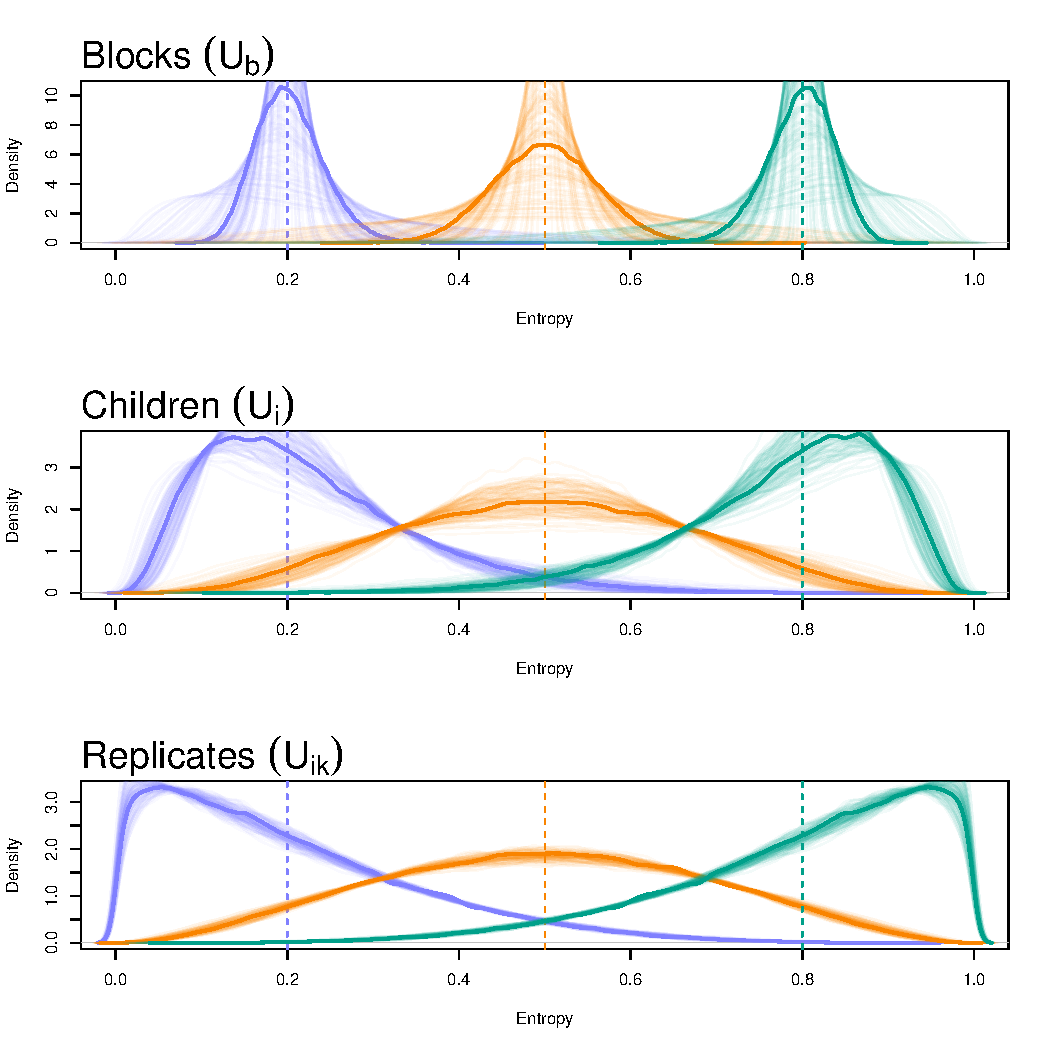
\includegraphics[width=0.6\linewidth]{variability_plot.pdf}
	\caption[Model 10, posterior predictive: variability present in the data]{Model 10, posterior predictive: variability present in the data. Distributions are plotted on the entropy replicates scale, considering three different averages: $\mu=0.2$, $\mu=0.5$, and $\mu=0.8$ (discontinuous lines). Thick solid lines represent the marginal distribution, thin solid lines depict $100$ random posterior samples.}
	\label{fig:variability}
\end{figure}
%
%
%###############################
\subsection{About our hypothesis} \label{sS:results_hypothesis}
%###############################
%
The current research used the Information-Theoretic Approach \citep{Anderson_2008, Chamberlain_1965} for model selection and inference. The application of the approach required: (i) the expression of the research hypothesis into statistical models, (ii) the selection of the most plausible models, and (iii) to produce inferences based on one or multiple selected models. The first requirement of the approach is covered in sections \ref{sS:causal_frame} and \ref{sS:stat_analysis}, and expanded in supplementary section \ref{sSA:model_details}. Here we use the results of the second requirement, detailed in the supplementary section \ref{ssSA:model_selection}, to produce the final inferences. 

As detailed in the supplementary section, the final conclusions of our research will be drawn from the comparisons of two models: (i) a no interaction model, with one estimated `sample size' (model 3), and (ii) a full interaction model, with one estimated `sample size' (model 10). The former is selected because it is the model with highest probabilistic support. The latter is considered because it encompasses the remaining highest supported models. Furthermore, no \textit{robust} models are inspected, as we prefer a more parsimonious depiction of our hypothesis. Table \ref{tab:results} summarizes the parameters posterior estimates and contrasts of interest. 
%
\begin{table}[h!]
	\centering
	\begin{tabular}{|cccccccccccc|} 
		\hline
		& \multicolumn{3}{c}{} & \multicolumn{2}{c}{CI} & & \multicolumn{2}{c}{HPDI} & & \multicolumn{2}{c|}{}\\[0.5ex]
		\cline{5-6} \cline{8-9}
		Parameter & Mean & SD & & $2.5\%$ & $97.5\%$ & & $2.5\%$ & $97.5\%$ & & n eff. & Rhat \\[0.5ex] 
		\hline\hline
		\rowcolor{gray}
		\multicolumn{12}{|l|}{ \textbf{Model 3: No interaction (one `size')} } \\
		\multicolumn{12}{|l|}{ \textbf{parameters:} } \\
		\texttt{a} & 0.179 & 0.189 & & -0.197 & 0.554 & & -0.198 & 0.552 & & 3'677.705 & 1.001\\
		\texttt{bP[2]} & -0.117 & 0.166 & & -0.439 & 0.207 & & -0.440 & 0.202 & & 1'738.855 & 1.000 \\
		\texttt{bA} & 0.432 & 0.141 & & 0.154 & 0.715 & & 0.170 & 0.723 & & 1'815.243 & 1.001 \\
		\texttt{aHS[1]} & 0.284 & 0.235 & & -0.178 & 0.761 & & -0.203 & 0.728 & & 2'719.833 & 1.000 \\
		\texttt{aHS[2]} & 0.116 & 0.217 & & -0.303 & 0.537 & & -0.304 & 0.537 & & 2'646.671 & 1.000 \\
		\multicolumn{12}{|l|}{ \textbf{constrast:} } \\
		\texttt{aHS[2]-aHS[1]} & -0.168 & 0.246 & & -0.661 & 0.371 & & -0.650 & 0.324 & & n.a. & n.a. \\
		\multicolumn{12}{|l|}{ } \\
		\rowcolor{gray}
		\multicolumn{12}{|l|}{ \textbf{Model 10: Full interaction (one `size')} } \\
		\multicolumn{12}{|l|}{ \textbf{parameters:} } \\
		\texttt{a} & 0.217 & 0.179 & & -0.142 & 0.562 & & -0.118 & 0.580 & & 3'902.629 & 0.999 \\
		\texttt{bP[2]} & -0.122 & 0.173 & & -0.457 & 0.220 & & -0.460 & 0.216 & & 1'659.639 & 1.002 \\
		\texttt{bAHS[1]} & 0.435 & 0.157 & & 0.127 & 0.745 & & 0.123 & 0.741 & & 1'477.460 & 1.000 \\
		\texttt{bAHS[2]} & 0.237 & 0.177 & & -0.119 & 0.596 & & -0.089 & 0.615 & & 1'844.785 & 1.001 \\
		\texttt{aEHS[1,1]} & 0.183 & 0.278 & & -0.358 & 0.726 & & -0.349 & 0.729 & & 2'524.451 & 1.000 \\
		\texttt{aEHS[2,2]} & 0.212 & 0.241 & & -0.259 & 0.684 & & -0.259 & 0.684 & & 2'418.275 & 0.999 \\
		\texttt{aEHS[3,2]} & 0.077 & 0.245 & & -0.402 & 0.547 & & -0.383 & 0.561 & & 3'015.559 & 0.999 \\
		\texttt{aEHS[4,2]} & 0.007 & 0.269 & & -0.522 & 0.530 & & -0.547 & 0.499 & & 3'268.043 & 1.000 \\
		\multicolumn{12}{|l|}{ \textbf{contrast:} } \\
		\texttt{bAHS[2]-bAHS[1]} & -0.197 & 0.208 & & -0.600 & 0.213 & & -0.590 & 0.223 & & n.a. & n.a. \\
		\texttt{aEHS[2,2]-aEHS[1,1]} & 0.029 & 0.352 & & -0.673 & 0.723 & & -0.714 & 0.682 & & n.a. & n.a. \\
		\texttt{aEHS[3,2]-aEHS[1,1]} & -0.106 & 0.365 & & -0.823 & 0.607 & & -0.822 & 0.609 & & n.a. & n.a. \\
		\texttt{aEHS[4,2]-aEHS[1,1]} & -0.176 & 0.380 & & -0.906 & 0.568 & & -0.928 & 0.535 & & n.a. & n.a. \\
		\texttt{aEHS[3,2]-aEHS[2,2]} & -0.135 & 0.299 & & -0.719 & 0.453 & & -0.730 & 0.439 & & n.a. & n.a. \\
		\texttt{aEHS[4,2]-aEHS[2,2]} & -0.205 & 0.344 & & -0.888 & 0.453 & & -0.902 & 0.430 & & n.a. & n.a. \\
		\texttt{aEHS[4,2]-aEHS[3,2]} & -0.070 & 0.344 & & -0.744 & 0.612 & & -0.735 & 0.617 & & n.a. & n.a. \\
		\hline
		\multicolumn{12}{l}{\footnotesize{CI = compatibility interval}} \\
		\multicolumn{12}{l}{\footnotesize{HDPI = highest posterior density interval}} \\
		\multicolumn{12}{l}{\footnotesize{n eff. = effective number samples}} \\
		\multicolumn{12}{l}{\footnotesize{Rhat = Gelman-Rubin diagnostic}} \\
		\multicolumn{12}{l}{\footnotesize{n.a. = not available / not applicable}} \\
		\multicolumn{12}{l}{\footnotesize{[1] = NH children, [2] = HI/CI children}} \\
		\multicolumn{12}{l}{\footnotesize{[1,i] = NH children, [2,i] = genetic, [3,i] = CMV infection, [4,i] = unknown etiology}} \\
	\end{tabular}
	\caption[Selected statistical models: results]{Selected statistical models: results.}
	\label{tab:results}
\end{table}

Before providing any parameter interpretation, it is important to highlight an statistical issue that will permeate all of our inferences. As it is detailed in section \ref{sS:results_variability}, with our current data size and given the large amount of variability registered at the children and replicates levels, the models are not able to produce unequivocal null hypothesis rejections for most of the parameters estimates, at a confidence level of $95\%$, i.e. the CI and HPDI will almost always include the zero value. This is particularly important, as rejecting the null hypothesis of certain parameters and contrast of interest provides unambiguous evidence for the current research hypothesis.

However, we consider that even when particular null hypothesis cannot be rejected, the models are still able show some preliminary evidence of effects and their direction. Given that parameter estimation under the Bayesian framework does not return parameters' point estimates, but rather the posterior distribution of possible values, we can still evaluate the amount of evidence towards a specific effect and its direction. In a complementary way, supplementary section \ref{ssSA:model_simulation} reveal that our models are also able to affirm the estimate values with at least $60\%$ power, depending on the estimates magnitudes, i.e. the models can correctly estimate values different from zero, when such alternative hypothesis is true. 

In that sense, we will continue interpreting the parameters, providing evidence on the directionality of the effects. Nevertheless, the reader should be cautious into understanding the CI and HPDI indicate that our data size might still not be enough, to ultimately define the direction of some effects with a certain level of confidence (usually $95\%$), and further observations at the children level might still be needed.

Considering the previous, for \textbf{\textit{hearing status}}, model three reveals that HI/CI children have a modest lower level of \textit{speech intelligibility}, compared to their NH counterparts (\texttt{aHS[2]-aHS[1]}). Notice the CI and HPDI include the value of zero, and therefore, null hypothesis rejections at a $95\%$ confidence level cannot be made. However, the posterior distribution of the contrast reveal that $76.8\%$ of the estimates are unequivocally below zero (\texttt{aHS[2]-aHS[1]} $< 0$). In this sense, the result seem to mildly support previous evidence on the matter \cite{Nicholas_et_al_2007, Castellanos_et_al_2014, Chin_et_al_2014, Geers_et_al_2016, Freeman_et_al_2017, Duchesne_et_al_2019, Grandon_et_al_2020}. 

Nevertheless, model ten paints a more nuanced story considering the \textbf{\textit{etiology}} of the disease. The contrasts of the model reveal that HI/CI children with genetic etiology manage to reach similar levels of \textit{intelligibility} as NH children (\texttt{aEHS[2,2]-aEHS[1,1]}). However, the same cannot be said when the hearing impairment is caused either by CMV infection (\texttt{aEHS[3,2]-aEHS[1,1]}) or other unknown causes (\texttt{aEHS[4,2]-aEHS[1,1]}). The posterior distribution of the aforementioned contrasts show the estimates are distinctly below zero with a probability of $62.4\%$ and $68\%$, respectively.

About the former result, we theorize a intuitive explanation. Since hearing loss is a brain issue, rather than ear issue \cite{Flexer_2011}, as children with genetic causes grow developing their language using the hearing apparatus, they grow constructing effective auditory neural pathways that benefit from the new hearing input from the start, even when that input is slightly degraded \cite{Drennan_et_al_2008}. However, the same cannot be said for other etiology status. What is hinted is that, a child with other etiology might need to `re-wire' his(her) auditory neural connections in order to fully take advantage of the new hearing signal. This is particularly important, if we consider these children are trying to achieve this `re-wiring' process, during an important maturing stage of the brain cortex (first twelve months) \cite{Flexer_2011}.

In relation to \textbf{\textit{hearing age}}, model three reveals what we initially expected: the factor is one of the main determinants for the increase in children's \textit{speech intelligibility}, showing statistically significant moderate effects (\texttt{bA}) \cite{Cohen_1988, Sawilowsky_2009}. However, model ten offers preliminary evidence contrary to what was previously found \cite{Boonen_et_al_2021}, indicating there is a difference in the evolution of \textit{intelligibility} between HI/CI and NH children (\texttt{bAHS[2]-bAHS[1]}). The posterior distribution of the contrast show $83.1\%$ of the estimates are unequivocally below zero. We intuit the latter result have two possible complementary explanations, either: (i) the children develop their language differently at different stages of their (\textit{hearing}) age \cite{Flexer_2011}, or (ii) given that the hearing signal provided by the apparatus is degraded \cite{Drennan_et_al_2008}, HI/CI children might take longer to achieve similar levels of \textit{intelligibility} than their NH counterparts.

Finally, for \textbf{\textit{pure tone average}}, we see both models support our initial hypothesis: HI/CI children with severe hearing loss, as accounted by the variable, develop their language at a slower rate than their NH counterparts (\texttt{bP[2]}). Notice again that $95\%$ confidence null hypothesis rejections cannot be made. However, the posterior distribution of the parameter reveal the estimates are unequivocally below zero with approximately $76\%$ probability (\texttt{bP[2]} $< 0$). Therefore, from perspective of effect sizes \cite{Cohen_1988, Sawilowsky_2009}, the estimates can be considered small in magnitude, but present nonetheless.

More interestingly still is that this results couple rather well with the second explanation for the effects of \textit{hearing age}, i.e. the more degraded the signal a child receives, either because of the apparatus or the severity of their hearing-impairment, the slower the \textit{speech intelligibility} evolves. 
%
%
%###############################
\subsection{The speech intelligibility scale} \label{sS:results_scales}
%###############################
%
As previously stated, one of the main benefits of the current methodology is that we can `construct' an \textit{intelligibility} score of the sampled children, which in turn, allow us to test different hypothesis and even make individual comparisons at the appropriate level. See supplementary section \ref{sSA:SI} for the appropriate interpretation of the scores.

Figure \ref{fig:predictive2} depicts the estimated \textit{true} entropy and \textit{speech intelligibility} scores per child. Three points can be highlighted from the figure. First, from the horizontal discontinuous lines, we can clearly assess that on average NH children have a modest higher level of intelligibility (lower entropy) than the HI/CI counterparts. However, given the children's variability, we cannot reject the hypothesis that HI/CI have similar levels than the NH children, as one can notice from the overlapping shaded areas of both groups. 

Second, the figure reveals there is some inherited uncertainty on the score estimates, resulting from using entropy replicates as a tool for measuring \textit{speech intelligibility}. The latter can be observed from the vertical lines, describing the highest posterior density intervals for the \textit{intelligibility} of each child. We argue this last trait is one of the main strengths of the method, as it allow us to not only make individual comparisons, but also consider the inherited (un)certainty of the comparison.

Third and final, the non-linear relationship between \textit{speech intelligibility} and the \textit{true} entropy scale is clearly noticed in the HPD intervals, where lowest/highest entropy values are paired with narrower intervals. Clear examples of this can be observed at the top panel of figure \ref{fig:predictive2}, where children $20$ and $25$ show narrower intervals at the lowest part of the scale, while child $6$ shows the analogous at the highest end of the same. The previous behavior is expected under non-linear statistical models. Nevertheless, this particular trait has an intuitive interpretation under our specific application, i.e. we can be more certain of the children's \textit{true} entropy values at the extreme of the hypothetical construct (either zero or one), rather than in the middle part of the scale.
%
%
\begin{figure}[!h]
	\centering
	\begin{tabular}{@{}@{}}
		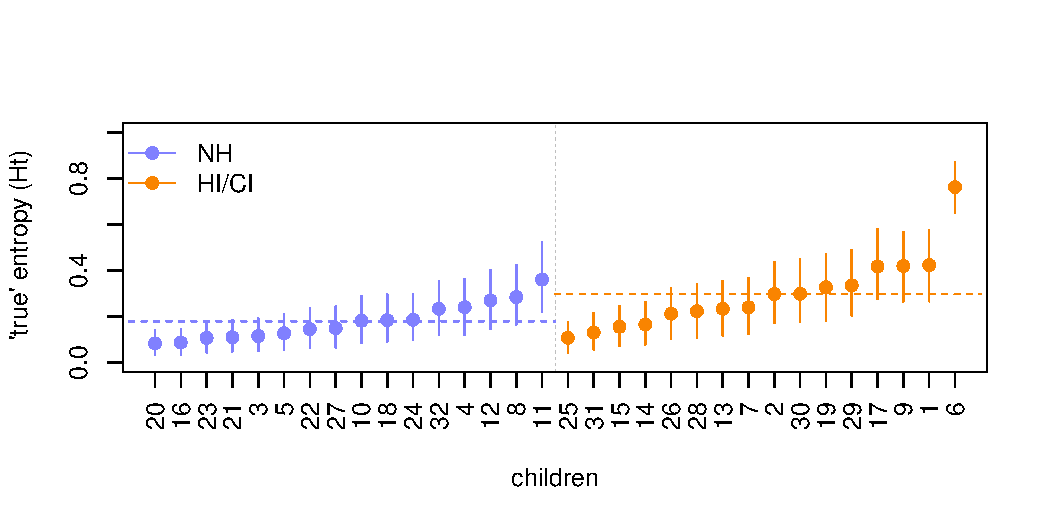
\includegraphics[trim=0 15 0 50, clip, width=0.65\textwidth]{posterior_predictive_real2_1.pdf} \\
		%trim=left lower right upper
		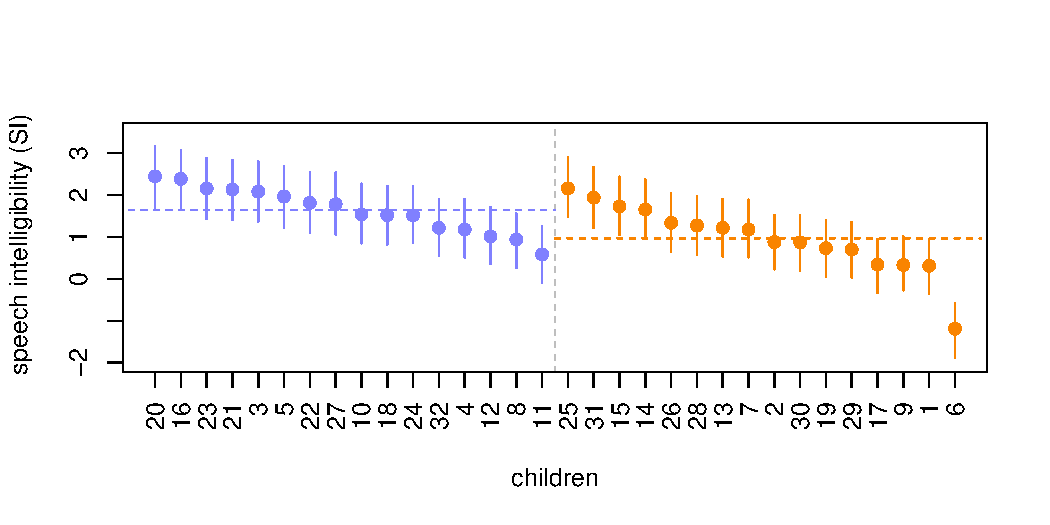
\includegraphics[trim=0 15 0 40, clip,, width=0.65\textwidth]{posterior_predictive_real2_2.pdf}
	\end{tabular}
	\caption[Model 10, posterior predictive: \textit{true} entropy and \textit{speech intelligibility} scales]{Model 10, posterior predictive: \textit{true} entropy and \textit{speech intelligibility} scales. Colored circles represent mean values per \textit{hearing status} group. Thin vertical continuous lines depict $95\%$ highest posterior density intervals (HDPI). Thin horizontal discontinuous lines represent the marginal average for the \textit{hearing status} group. Shaded area represent the marginal averages $95\%$ confidence interval.}
	\label{fig:predictive2}
\end{figure}
%
%
%###############################
\subsection{Posterior predictive} \label{sS:results_posterior}
%###############################
%
The posterior predictive results give us with a tool to assess how good our models were to reconstruct the observed data. Figure \ref{fig:predictive1} shows our full interaction model managed to `recreate' our data, while also provided the (un)certainty around the entropy replicates. The latter was shown in two ways: (i) through the point estimates and HPD intervals for the \textit{true} entropy scale (red points and horizontal lines), and (ii) though the expected estimated marginal and sampled distributions for the entropy replicates (thick and thin solid distribution lines, respectively).
%
%
%###############################
\subsection{Influential observations} \label{sS:results_outliers}
%###############################
%
Finally, implementing the statistical models under the Bayesian framework provide us with one last advantage: we were able to identify influential observations that might sway our estimates, under our model framework \citep{McElreath_2020}. We argue this method is preferable, as the identification of influential observations through preliminary or univariate procedures might lead to erroneous exclusion of information, ultimately damaging our research inferences. See supplementary section \ref{ssSA:preprocessing} for more details.

Figure \ref{fig:outliers} provides an overview of the identified high-leverage observations (pair child, utterance). Model ten reveals some observations for children 8, 10, and 15 can be deemed prominent. The first two were NH children, while the last was an HI/CI analogue. 

After a careful inspection, the only similitude between these observations was that all of them registered the lowest replicate values observed in the sample ($0.007$ for child 8, and zero for the remaining two). Therefore, it makes sense our model found these points `surprising', as they are mostly out of the expected range for the outcome. The latter is particularly true for child $15$, as it is not expected that an HI/CI child have traits of perfect \textit{intelligibility}, as the replicate seem to indicate. 

However, notice additionally that even with their presence, no further evidence was found in favor of \textit{robust} models over other more parsimonious iterations of our research hypothesis (see supplementary section \ref{ssSA:model_selection}). As a result, none of these observation were excluded from the analysis, but they were identified and can be further investigated.
%
%
\begin{figure}[!h]
	\centering
	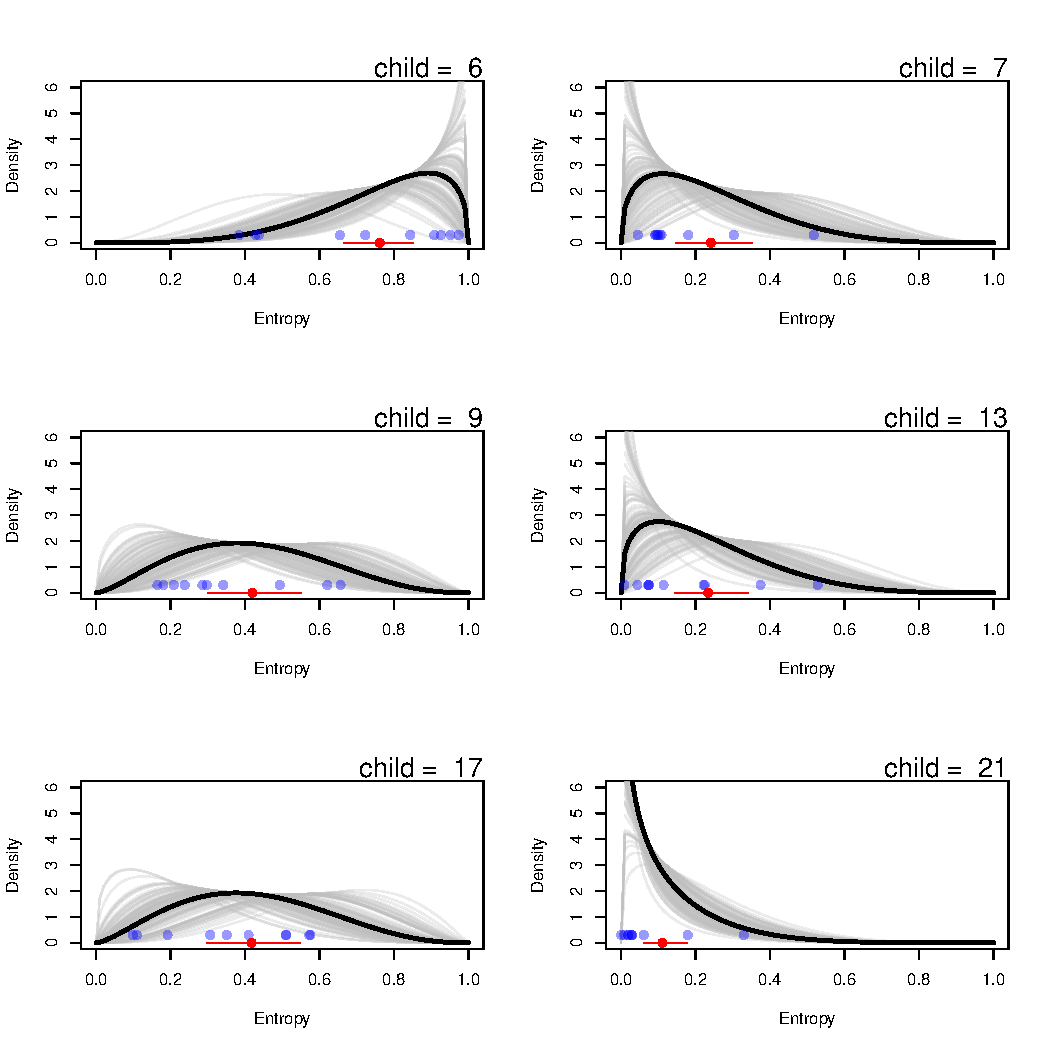
\includegraphics[trim=0 10 0 25, clip, width=0.65\linewidth]{posterior_predictive_real1.pdf}
	%trim=left lower right upper
	\caption[Model 10, posterior predictive: entropy replicates, \textit{true} entropy, and distributions]{Model 10, posterior predictive: entropy replicates, \textit{true} entropy, and distributions. Colored points represent the entropy replicates per \textit{hearing status} group. Red points with lines represent the mean \textit{true} entropy with $95\%$ highest posterior density interval (HPDI). Thick solid line represents the marginal distribution, thin solid lines depicts $100$ random posterior samples for the distributions.}
	\label{fig:predictive1}
\end{figure}
%
%
\begin{figure}[!h]
	\centering
	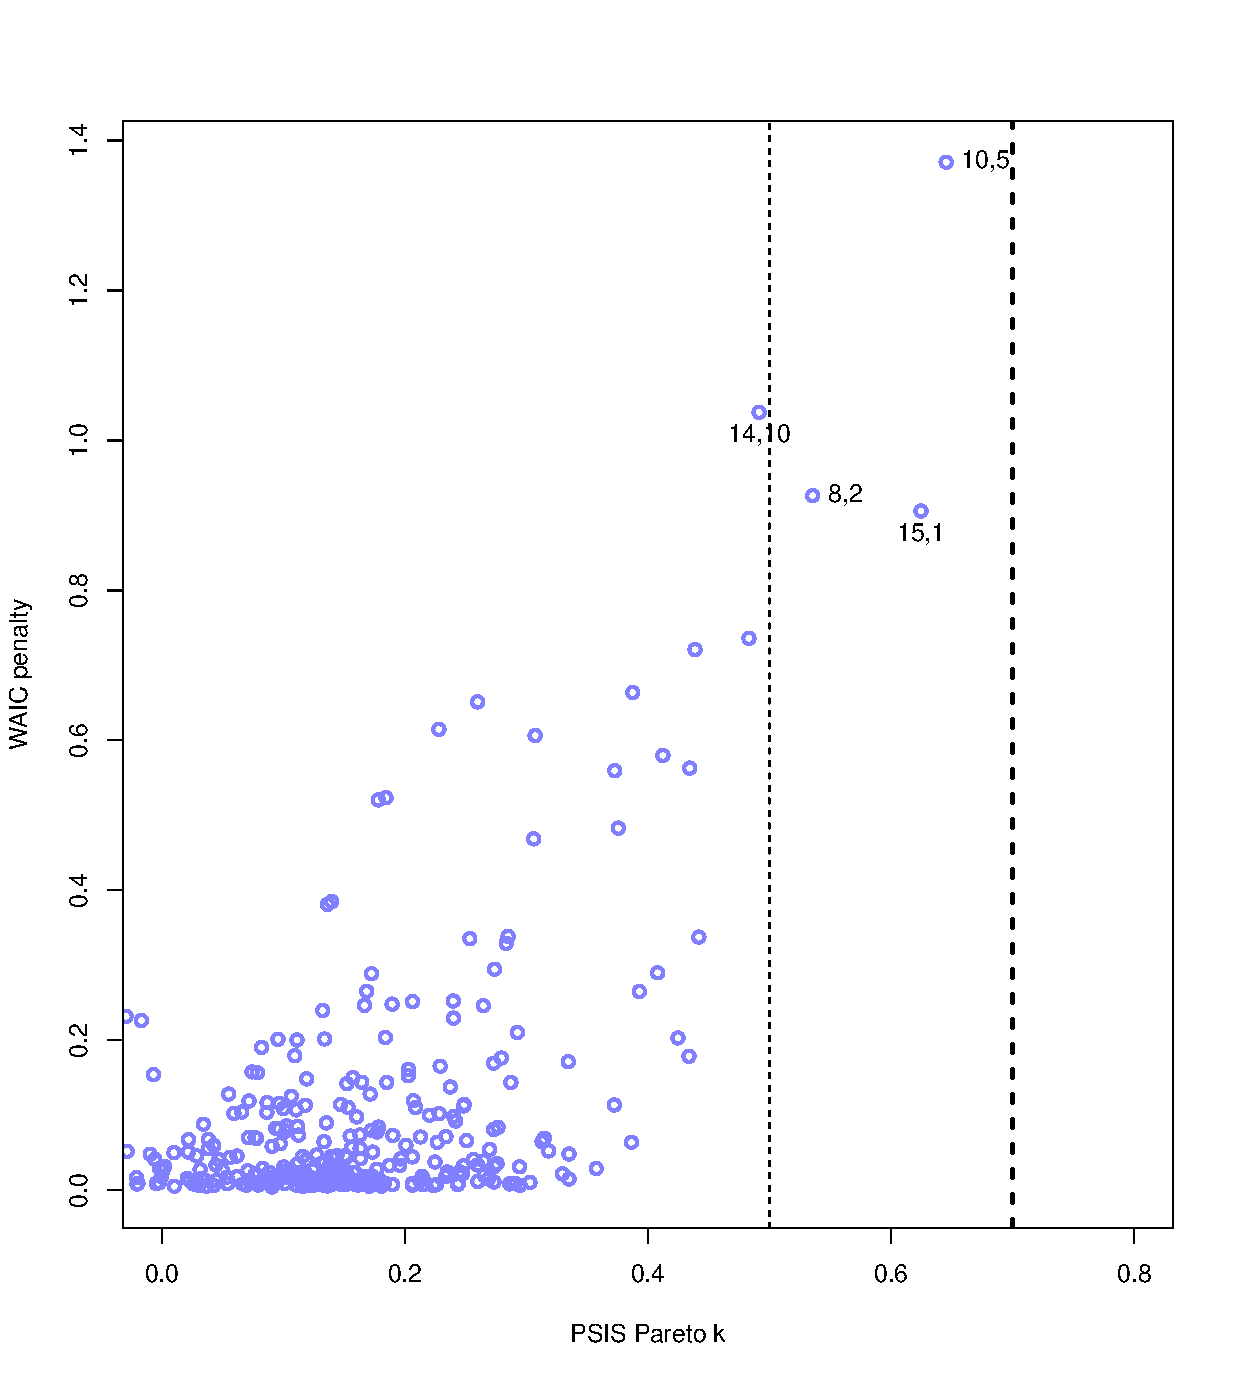
\includegraphics[trim=0 10 0 55, clip, width=0.50\linewidth]{outliers.pdf}
	%trim=left lower right upper
	\caption[Model 10, influential observations]{Model 10, influential observations. Pairs child, utterance are reported for specific observations. Thin and thick discontinuous lines indicate the minimum and extreme recommended threshold of identification ($0.5$ and $0.7$, respectively).}
	\label{fig:outliers}
\end{figure}
%
%